% Тип документа
\documentclass[a4paper,12pt]{extarticle}

% Шрифты, кодировки, символьные таблицы, переносы
\usepackage{cmap}
\usepackage[T2A]{fontenc}
\usepackage[utf8x]{inputenc}
\usepackage[russian]{babel}

% Это пакет -- хитрый пакет, он нужен но не нужен
\usepackage[mode=buildnew]{standalone}

\usepackage
	{
		% Дополнения Американского математического общества (AMS)
		amssymb,
		amsfonts,
		amsmath,
		amsthm,
		physics,
		% misccorr,
		% 
		% Графики и рисунки
		wrapfig,
		graphicx,
		subcaption,
		float,
		tikz,
		tikz-3dplot,
		caption,
		csvsimple,
		color,
		booktabs,
		pgfplots,
		pgfplotstable,
		geometry,
		% 
		% Таблицы, списки
		makecell,
		multirow,
		indentfirst,
		%
		% Интегралы и прочие обозначения
		ulem,
		esint,
		esdiff,
		% 
		% Колонтитулы
		fancyhdr,
	}  

\usepackage{xcolor}
\usepackage{hyperref}

 % Цвета для гиперссылок
\definecolor{linkcolor}{HTML}{000000} % цвет ссылок
\definecolor{urlcolor}{HTML}{799B03} % цвет гиперссылок
 
\hypersetup{pdfstartview=FitH,  linkcolor=linkcolor,urlcolor=urlcolor, colorlinks=true}
% Обводка текста в TikZ
\usepackage[outline]{contour}

% Увеличенный межстрочный интервал, французские пробелы
\linespread{1.3} 
\frenchspacing 

 
\usetikzlibrary
	{
		decorations.pathreplacing,
		decorations.pathmorphing,
		patterns,
		calc,
		scopes,
		arrows,
		fadings,
		through,
		shapes.misc,
		arrows.meta,
		3d,
		quotes,
		angles,
		babel
	}


\tikzset{
	force/.style=	{
		>=latex,
		draw=blue,
		fill=blue,
				 	}, 
	%				 	
	axis/.style=	{
		densely dashed,
		blue,
		line width=1pt,
		font=\small,
					},
	%
	th/.style=	{
		line width=1pt},
	%
	acceleration/.style={
		>=open triangle 60,
		draw=magenta,
		fill=magenta,
					},
	%
	inforce/.style=	{
		force,
		double equal sign distance=2pt,
					},
	%
	interface/.style={
		pattern = north east lines, 
		draw    = none, 
		pattern color=gray!60,
					},
	cross/.style=	{
		cross out, 
		draw=black, 
		minimum size=2*(#1-\pgflinewidth), 
		inner sep=0pt, outer sep=0pt,
					},
	%
	cargo/.style=	{
		rectangle, 
		fill=black!70, 
		inner sep=2.5mm,
					},
	%
	caption/.style= {
		midway,
		fill=white!20, 
		opacity=0.9
					},
	%
	}

\newenvironment{tikzpict}
    {
	    \begin{figure}[htbp]
		\centering
		\begin{tikzpicture}
    }
    { 
		\end{tikzpicture}
		% \caption{caption}
		% \label{fig:label}
		\end{figure}
    }


\newcommand{\vbLabel}[3]{\draw ($(#1,#2)+(0,5pt)$) -- ($(#1,#2)-(0,5pt)$) node[below]{#3}}
\newcommand{\vaLabel}[3]{\draw ($(#1,#2)+(0,5pt)$) node[above]{#3} -- ($(#1,#2)-(0,5pt)$) }

\newcommand{\hrLabel}[3]{\draw ($(#1,#2)+(5pt,0)$) -- ($(#1,#2)-(5pt,0)$) node[right, xshift=1em]{#3}}
\newcommand{\hlLabel}[3]{\draw ($(#1,#2)+(5pt,0)$) node[left, xshift=-1em]{#3} -- ($(#1,#2)-(5pt,0)$) }



\newcommand\zi{^{\,*}_i}
\newcommand\sumn{\sum_{i=1}^{N}}

\tikzset{
	coordsys/.style={scale=1.8,x={(1.1cm,-0cm)},y={(0.5cm,1cm)}, z={(0cm,0.8cm)}},
	coordsys/.style={scale=1.5,x={(0cm,0cm)},y={(1cm,0cm)}, z={(0cm,1cm)}}, 
	coordsys/.style={scale=1.5,x={(1cm,0cm)},y={(0cm,1cm)}, z={(0cm,0cm)}}, 
}

\usepgfplotslibrary{units}


% Draw line annotation
% Input:
%   #1 Line offset (optional)
%   #2 Line angle
%   #3 Line length
%   #5 Line label
% Example:
%   \lineann[1]{30}{2}{$L_1$}

\newcommand{\lineann}[4][0.5]{%
    \begin{scope}[rotate=#2, blue,inner sep=2pt, ]
        \draw[dashed, blue!40] (0,0) -- +(0,#1)
            node [coordinate, near end] (a) {};
        \draw[dashed, blue!40] (#3,0) -- +(0,#1)
            node [coordinate, near end] (b) {};
        \draw[|<->|] (a) -- node[fill=white, scale=0.8] {#4} (b);
    \end{scope}
}

\newcommand{\lineannn}[4][0.5]{%
    \begin{scope}[rotate=#2, blue,inner sep=2pt, ]
        \draw[dashed, blue!40] (0,0) -- +(0,#1)
            node [coordinate, near end] (a) {};
        \draw[dashed, blue!40] (#3,0) -- +(0,#1)
            node [coordinate, near end] (b) {};
        % \draw[color=white, color=blue] (a) -- node[fill=white, scale=0.8] {#4} (b);
        \draw[->|] (a)++(-0.3,0) -- (a);
        \draw[->|] (b)++(0.3,0) coordinate (xx) -- (b);
        \draw (xx) node[fill=white, scale=0.8, right] {#4};
    \end{scope}
}

% Круговая стрелка относительно центра (дуга из центра)
\tikzset{
  pics/carc/.style args={#1:#2:#3}{
    code={
      \draw[pic actions] (#1:#3) arc(#1:#2:#3);
    }
  },
  dash/.style={
  	dash pattern=on 5mm off 5mm
  }
}

% Среднее <#1>
\newcommand{\mean}[1]{\langle#1\rangle}

\pgfplotsset{
    % most recent feature set of pgfplots
    compat=newest,
}

% const прямым шрифтом
\newcommand\ct[1]{\text{\rmfamily\upshape #1}}
\newcommand*{\const}{\ct{const}}


\usepackage[europeanresistors,americaninductors]{circuitikz}

% Style to select only points from #1 to #2 (inclusive)
\pgfplotsset{select/.style 2 args={
    x filter/.code={
        \ifnum\coordindex<#1\def\pgfmathresult{}\fi
        \ifnum\coordindex>#2\def\pgfmathresult{}\fi
    }
}}


\usepackage{array}
\usepackage{pstool}


%%%%%%%%%%%%%%%%%%%%%%%%%%%%%%%%%%%%%%%%%%%%%%%%%
\makeatletter
\newif\if@gather@prefix 
\preto\place@tag@gather{% 
  \if@gather@prefix\iftagsleft@ 
    \kern-\gdisplaywidth@ 
    \rlap{\gather@prefix}% 
    \kern\gdisplaywidth@ 
  \fi\fi 
} 
\appto\place@tag@gather{% 
  \if@gather@prefix\iftagsleft@\else 
    \kern-\displaywidth 
    \rlap{\gather@prefix}% 
    \kern\displaywidth 
  \fi\fi 
  \global\@gather@prefixfalse 
} 
\preto\place@tag{% 
  \if@gather@prefix\iftagsleft@ 
    \kern-\gdisplaywidth@ 
    \rlap{\gather@prefix}% 
    \kern\displaywidth@ 
  \fi\fi 
} 
\appto\place@tag{% 
  \if@gather@prefix\iftagsleft@\else 
    \kern-\displaywidth 
    \rlap{\gather@prefix}% 
    \kern\displaywidth 
  \fi\fi 
  \global\@gather@prefixfalse 
} 
\newcommand*{\beforetext}[1]{% 
  \ifmeasuring@\else
  \gdef\gather@prefix{#1}% 
  \global\@gather@prefixtrue 
  \fi
} 
\makeatother
%%%%%%%%%%%%%%%%%%%%%%%%%%%%%%%%%%%%%%%%%%%%%%%%%

\geometry		
	{
		left			=	2cm,
		right 			=	2cm,
		top 			=	3cm,
		bottom 			=	3cm,
		bindingoffset	=	0cm
	}

%%%%%%%%%%%%%%%%%%%%%%%%%%%%%%%%%%%%%%%%%%%%%%%%%%%%%%%%%%%%%%%%%%%%%%%%%%%%%%%



	%применим колонтитул к стилю страницы
\pagestyle{fancy} 
	%очистим "шапку" страницы
\fancyhead{} 
	%слева сверху на четных и справа на нечетных
\fancyhead[R]{\labauthors} 
	%справа сверху на четных и слева на нечетных
\fancyhead[L]{Отчёт по лабораторной работе №\labnumber} 
	%очистим "подвал" страницы
\fancyfoot{} 
	% номер страницы в нижнем колинтуле в центре
\fancyfoot[C]{\thepage} 

%%%%%%%%%%%%%%%%%%%%%%%%%%%%%%%%%%%%%%%%%%%%%%%%%%%%%%%%%%%%%%%%%%%%%%%%%%%%%%%

\renewcommand{\contentsname}{Оглавление}

\usepackage{tocloft}
% \renewcommand{\cftpartleader}{\cftdotfill{\cftdotsep}} % for parts
% \renewcommand{\cftsectiondotsep}{\cftdotsep}% Chapters should use dots in ToC
\renewcommand{\cftsecleader}{\cftdotfill{\cftdotsep}}
%\renewcommand{\cftsecleader}{\cftdotfill{\cftdotsep}} % for sections, if you really want! (It is default in report and book class (So you may not need it).
% ---------
% \newcommand{\cftchapaftersnum}{.}%
% \usepackage{titlesec}
% \titlelabel{\thetitle.\quad}
\usepackage{secdot}
\sectiondot{subsection}

\begin{document}

\def\labauthors{Карусевич А.А., Шиков А.П.}
\def\labgroup{440}
\def\labnumber{1}
\def\labtheme{Измерение статистических характеристик полупроводникового диода}
\renewcommand{\vec}{\mathbf}
\renewcommand{\phi}{\varphi}
\renewcommand{\hat}{\widehat}

\begin{titlepage}

\begin{center}

{\small\textsc{Нижегородский государственный университет имени Н.\,И. Лобачевского}}
\vskip 1pt \hrule \vskip 3pt
{\small\textsc{Радиофизический факультет}}

\vfill

{\Large Отчет по лабораторной работе №\labnumber\vskip 12pt\bfseries \labtheme}
	
\end{center}

\vfill
	
\begin{flushright}
	{Выполнили студенты \labgroup\ группы\\ \labauthors}%\vskip 12pt Принял:\\ Менсов С.\,Н.}
\end{flushright}
	
\vfill
	
\begin{center}
	Нижний Новгород, \the\year
\end{center}

\end{titlepage}



\section{Введение}
Физика контактных явлений служит основой разработки важнейших структурных элементов подавляющего большинства приборов современной микроэлектроники. В данной работе будут кратко изучены элементарные основы теории контактных явлений как на границе двух различных материалов, так и внутри одного и того же полупроводникового кристалла между областями с разным типом проводимости. Физические свойства подобных контактов широко используются для выпрямления тока и лежат в основе работы базовых элементов целого ряда полупроводниковых сверхвысокочастотных устройств и быстродействующих интегральных схем, а также полупроводниковой оптоэлектроники.

\section{Границы раздела между полупроводниками}
\subsection{Изотипный (униполярный) гомопереход}
Область электронного полупроводника, имеющую высокую концентрацию доноров, обозначают $"n^+"$. Если в полупроводнике n-типа создается область $n^+$, то говорят об $n^+-n$ переходе. 

Поскольку концентрация электронов в $n^+$ области больше, чем в n-области, то диффузионный ток будет направлен справа налево (рис.1). Он будет переносить электроны, пока не возникнет внутреннее поле (образованное ионами доноров и избыточными электронами) такой величины, при которой создаваемый им встречный дрейфовый ток не уравновесит ток диффузионный, т.е. пока не будет достигнуто динамическое равновесие. Зонная диаграмма и графики зависимости концентрации доноров и электронов от координаты в равновесном состоянии показаны на рис.1. 
\begin{figure}[h!]
	\centering
	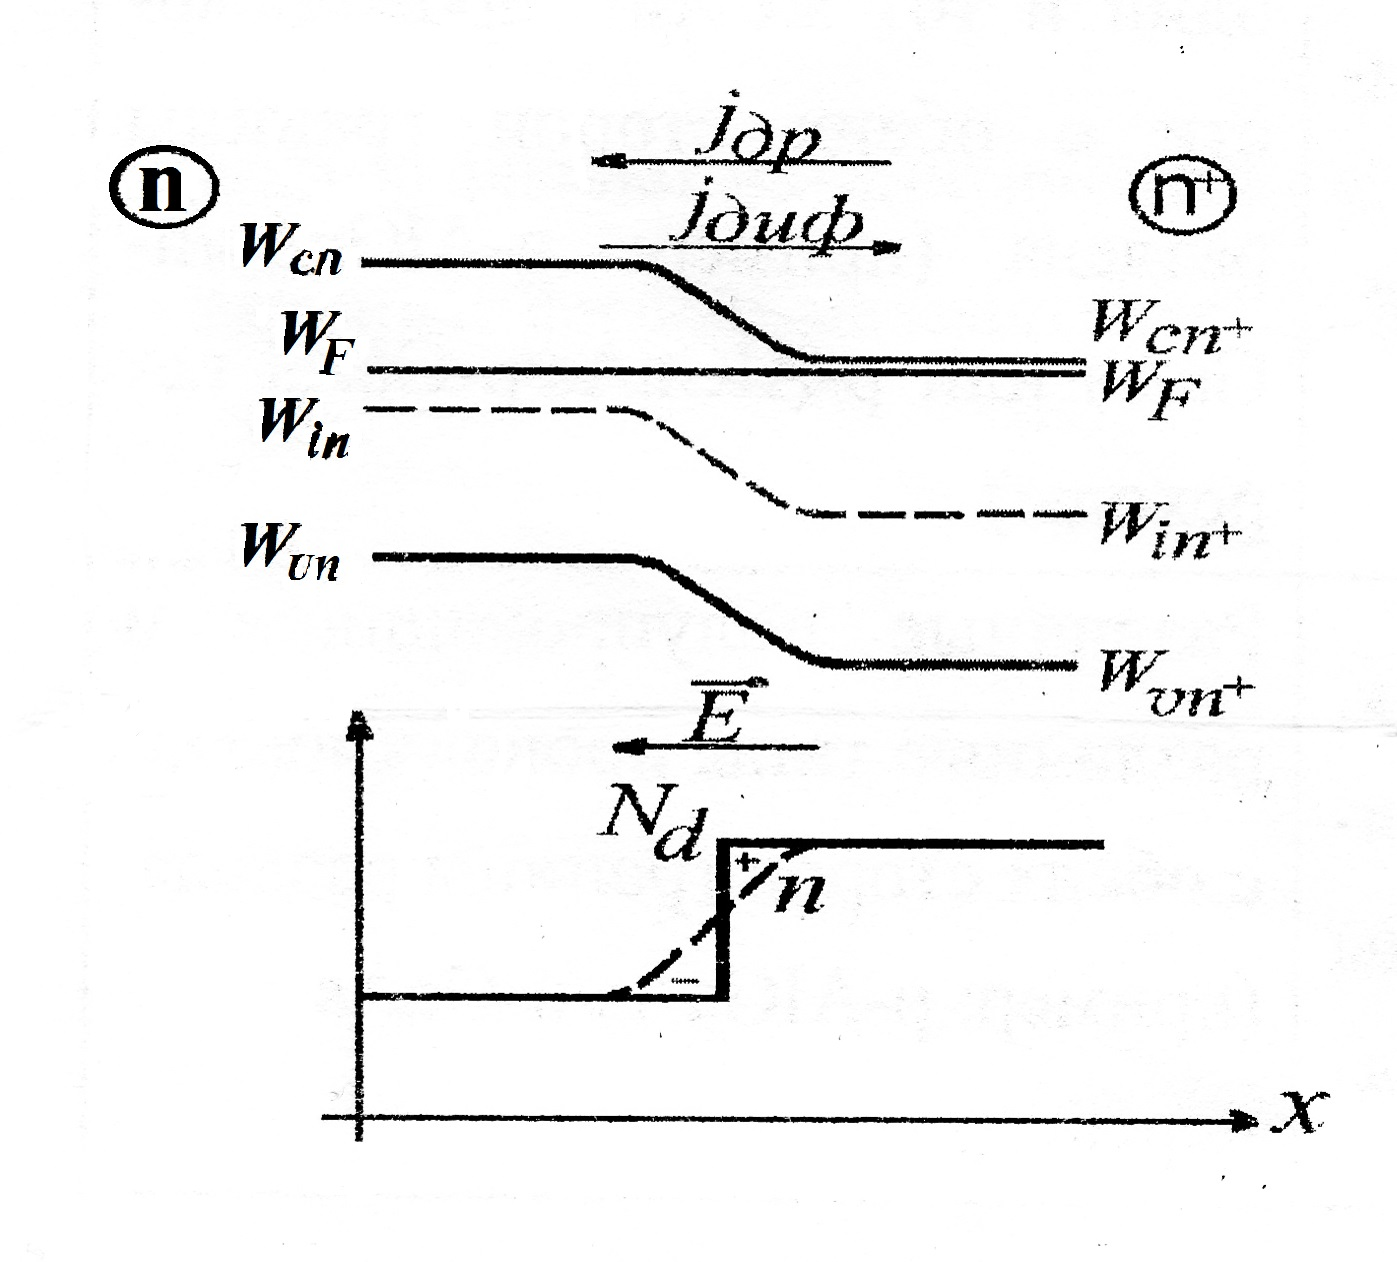
\includegraphics[width=0.35\linewidth]{fig/fig1.jpg}
	\caption{Энергетическая зонная диаграмма и график зависимостей концентрации доноров и электронов от координаты в $n^+-n$ переходе в состоянии равновесия}
	\label{fig:1}
\end{figure}

На практике чаще всего используют изотипные переходы с уровнями легирования обеих частей более $10^{16}-10^{17} \text{см}^{-3}$, поэтому высота барьера между правой и левой областями перехода имеет величину порядка нескольких kT, а электрическое сопротивление, обусловленное таким барьером, мало по сравнению с сопротивлениями остальных переходов.  
\subsection{Анизотипный (биполярный) гомопереход (p-n переход)}
Электронно-дырочным или p=n переходом называется приконтактная область между частями полупроводника с электронной (n)и дырочной (p) проводимостями. 

В зависимости от характера распределения примесей различают резкий (ступенчатый) и плавный p-n переходы. Рассмотрим резкий переход при условии $N_a \gg N_d$.

\subsubsection{Электронно-дырочный переход в равновесном состоянии}
В p-области концентрация дырок ($p_p$) - основных носителей заряда - значительно больше, чем в n-области. Поэтому они диффундируют в n-область, где будут неосновными носителями заряда ($p_n$). Благодаря интенсивной рекомбинации в некотором слое n-области, примыкающем к границе раздела, появится положительный объемный заряд, обусловленный ионами донорной примеси. Аналогично, диффузия и рекомбинация электронов будут сопровождаться образованием в p-области отрицательного объемного заряда ионов акцепторной примеси. Наличие объемного заряда вызывает появление встроенного электрического поля. Таким образом, на границе раздела между p- и n-областями появляется разность потенциалов, которую называют контактной $U_k$.

Электрическое поле, созданное в объединенной области ионами легирующей примеси, препятствует переходу через нее основных носителей заряда. Однако, это поле вызывает дрейфовый ток неосновных носителей, который направлен противоположно диффузионному току. В равновесном состоянии в отсутствие внешнего напряжения результирующий ток через переход равен нулю. Это означает, что силы электрического поля и силы, определяющее диффузию носителей заряда, уравновешивают друг друга. приконтактную область, где имеется электрическое поле, называют p-n переходом.

\subsubsection{Вольт-амперная характеристика p-n перехода}
Пусть к электронно-дырочному переходу подключен источник ЭДС таким образом, чтобы потенциальный барьер уменьшился. Такое подключение называется прямым и оно соответствует подсоединению источника плюсом к p-области и минусом к n-области. 

При прямом смещении из-за уменьшения потенциального барьера основные носители в областях p и n, имеющие наибольшую энергию, получат возможность преодолевать потенциальный барьер и проникать через него в области, где они оказываются неосновными и рекомбинируют. Эти избыточные неравновесные носители нарушат электронейтральность полупроводника вблизи перехода и вызовут в равном количестве приток основных носителей из глубины p- и n-областей. Скорость рекомбинации электронов и дырок конечна, поэтому неравновесные носители могут подвинуться вглубь полупроводника и глубина их проникновения значительно превысит толщину запорного слоя. При этом электронейтральность кристалла за пределами области объемного заряда не нарушается. 

Таким образом, при наложении внешнего напряжения в прямом направлении в результате инжекции  носителей через p-n переход будет протекать ток, величина которого будет нарастать с увеличением приложенного напряжения. при обратной полярности внешнего напряжения высота потенциального барьера увеличивается. Ток в этом случае определяется неосновными носителями заряда и незначителен по величине.

Вольт-амперная характеристика диода:
\begin{figure}[h!]
	\centering
	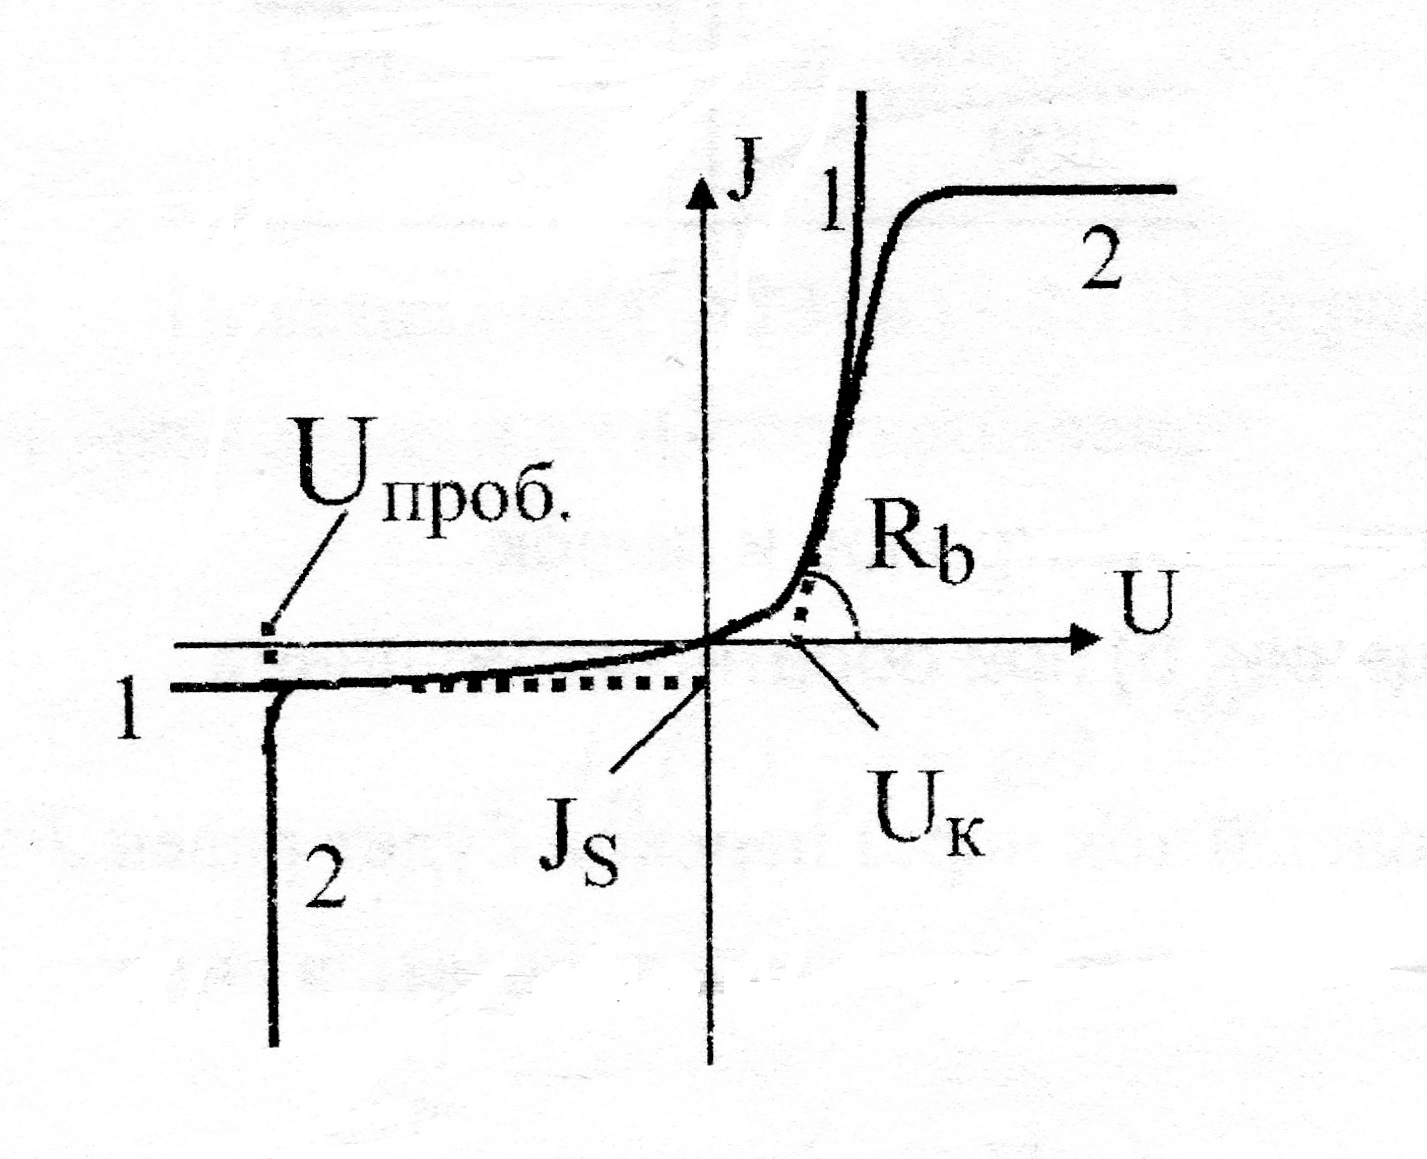
\includegraphics[width=0.5\linewidth]{fig/fig2.jpg}
	\caption{ВАХ p-n перехода: 1) идеальная; 2) реальная}
	\label{fig:2}
\end{figure}

Отличия от теоретической зависимости наблюдаются при увеличении прямого тока и при больших обратных напряжениях, когда имеет место резкое возрастание обратного тока и пробой перехода. 

У реального диода последовательно с сопротивлением p-n перехода имеется сопротивление базы (область с большей концентрацией примесей называют эмиттером, а с меньшей - базой). При больших прямых токах падение напряжения на этом сопротивлении соизмеримо с падением на переходе. С учетом сопротивления базы аналитическое выражение зависимости тока диода от приложенного к нему напряжения может быть представлено в виде:

\begin{gather}
	J=J_s[e^{(U/\varphi_T-JR_{\text{б}}/\varphi_T)}-1].
\end{gather}
где U - напряжение, приложенное к диоду, $R_{\text{б}}$ - сопротивление базы. 

Проведя логарифмирование и дифференцирование этого выражения, определим дифференциальное сопротивление в произвольной точке вольт-амперной характеристики:
\begin{gather}
	R_{\text{д}}=\dv{U}{J}=\frac{\varphi_T}{(J+J_s)}+R_{\text{б}}.
\end{gather}

Отсюда следует, что при малых токах дифференциальное сопротивление зависит главным образом от сопротивления p-n перехода. При больших токах дифференциальное сопротивление перехода мало и общее сопротивление определяется сопротивлением базы, т.е. зависимость от напряжения представляет собой линию, угол наклона которой пропорционален величине $R_{\text{д}}$. При дальнейшем увеличении прямого напряжения ток прибора выходит на насыщение. Причины этого явления зависят от конструкции прибора и определяются: насыщением зависимости скорости носителей заряда в сильных электрических полях, малой концентрацией носителей заряда при слабом легировании полупроводника, разогревом полупроводника протекающим током.

\subsubsection{Емкость электронно-дырочного перехода}
Всякий p-n переход по существу представляет собой систему двух проводников, разделенных слоем объемного заряда. Такая система подобна плоскому конденсатору. Опыт показывает, что полупроводниковые диоды обладают значительной емкостью. Емкость диода играет большую роль, ограничивая применение диодов на высоких частотах. изучение емкости перехода во многих случаях помогает исследовать структуру запирающего слоя и механизм выпрямления.

Ширина области объемного заряда:
\begin{gather}
	d=\sqrt{\frac{2\varepsilon \varepsilon_o(N_a+N_d)(U_k-U)}{eN_aN_d}}.
\end{gather} 

Видно, что ширина уменьшается с увеличением прямого (положительного) напряжения и увеличивается при обратном напряжении.

Изменение ширины области объемного заряда в связи с изменением напряжения приводит к изменению заряда в p- и n-областях. Поэтому p-n переход ведет себя подобно емкости. Эту емкость называют барьерной, т.к. она связана с образованием потенциального барьера между p- и n-областями. 
\begin{gather}
	C=S\frac{\varepsilon \varepsilon_o}{d}=S\sqrt{\frac{e\varepsilon \varepsilon_oN_aN_d}{2(N_a+N_d)(U_k-U)}},
\end{gather}
где S - площадь перехода.

В случае резко несимметричного p-n перехода, например, при $N_a \gg N_d$, переход расширяется в n-область и величина барьерной емкости не зависит от свойств p-области:
\begin{gather}
	C=S\sqrt{\frac{e\varepsilon \varepsilon_oN_d}{2(U_k-U)}}.
\end{gather}

Это выражение позволяет найти контактную разность потенциалов и концентрацию донорной примеси. График зависимости $\frac{1}{C^2}=f(U)$, изображенный на рис.3, отсекает на оси абсцисс отрезок, равный по величине $U_k$. Если известна зависимость $C=f(U)$, то на основании равенства (4) можно построить зависимость ширины объединенной области от приложенного напряжения.
\begin{figure}[h!]
	\centering
	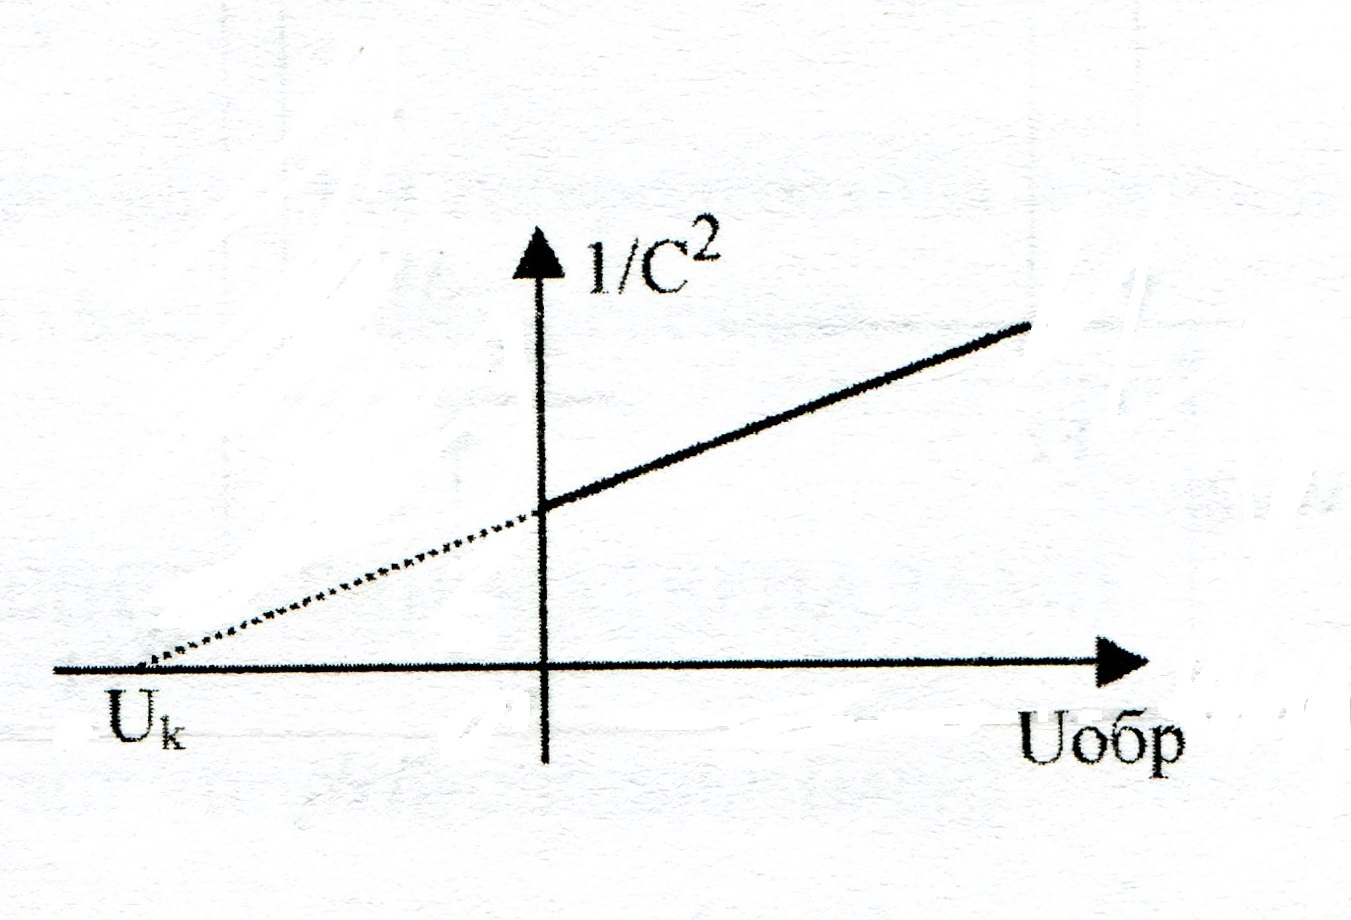
\includegraphics[width=0.5\linewidth]{fig/fig3.jpg}
	\caption{Вольт-фарадная характеристика p-n перехода(здесь $U_{\text{обр}}$ - обратное напряжение).}
	\label{fig:3}
\end{figure}

\section{Эквивалентные схемы диодов}
\begin{figure}[h!]
	\centering
	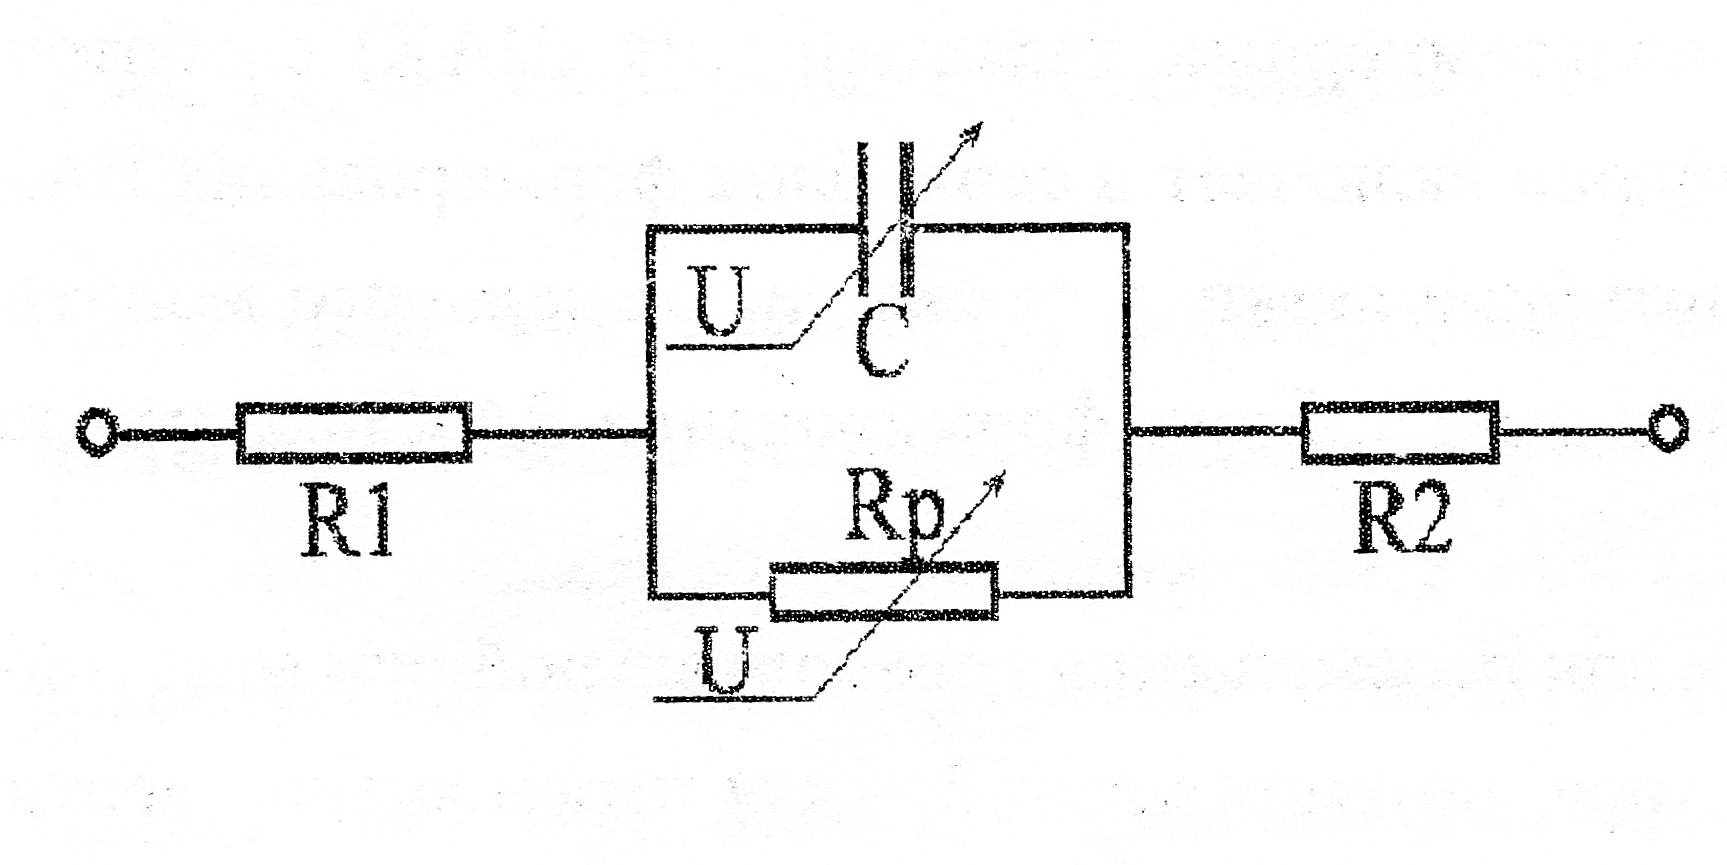
\includegraphics[width=0.5\linewidth]{fig/fig4.jpg}
	\caption{Эквивалентная схема диодов на основе p-n перехода, барьера Шоттки и МПД структуры}
	\label{fig:4}
\end{figure}

Здесь С - управляемая напряжением емкость перехода; U - величина напряжения, приложенного непосредственно к переходу (т.е. без учета падения напряжения на сопротивлениях R1 и R2); R1 и R2 - последовательные сопротивления областей материала по обе стороны от перехода; $R_p$ - управляемое напряжением сопротивление перехода или барьера Шоттки (определяется из ВАХ диодов).

\section{Экспериментальная часть}
\subsection{Экспериментальная установка}
Схема:
\begin{figure}[h!]
	\centering
	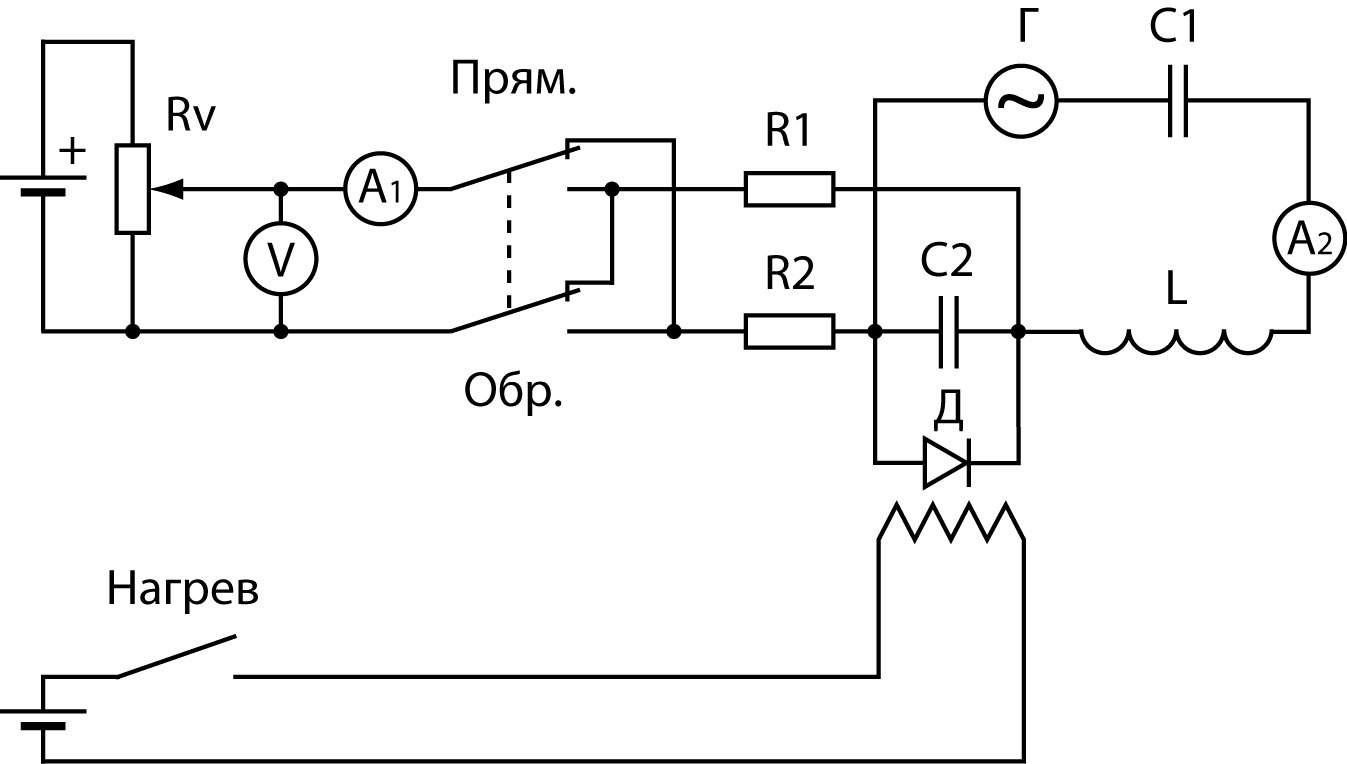
\includegraphics[width=0.5\linewidth]{fig/fig5.jpg}
	\caption{Схема экспериментальной установки}
	\label{fig:5}
\end{figure}

L=364 мкГн, $C_2$=37.9 пФ, S=1 мм$^2$.

В состав установки для измерения статических характеристик полупроводникового диода (рис. 6) производится на установке, состоящей из блока режимов (1) и высокочастотного генератора (2).
\begin{figure}[h!]
	\centering
	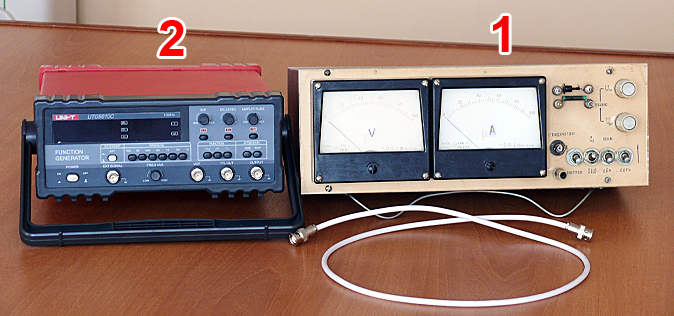
\includegraphics[width=0.6\linewidth]{fig/fig6.jpg}
	\caption{}
	\label{fig:6}
\end{figure}

\subsection{ВАХ диода при комнатной температуре}

% \subsection{Установка}
% Экспериментальная установка по наблюдению сигнала поглощения ЭПР собрана по схеме СВЧ-спектроскопии. Блок-схема радиоспектрометра ЭПР, используемого в данной работе, представленна на рис.1:
% \begin{figure}[h!]
% 	\centering
% 	\includegraphics[width=\linewidth]{fig/Sh.jpg}
% 	\caption{Блок-схема ЭПР-спектрометра}
% 	\label{fig:1}
% \end{figure}

% Рассмотрим кратко работу ЭПР-спектрометра. Сигнал с клистронного генератора, который является источником излучения высокочастотного поля $\vec{H_1}(\lambda \approx$ 3 см), через ферритовый вентиль поступает во входное плечо двойного тройника. двойной тройник, собранный по мостовой схеме, служит для разделения мощности на две равные части. Одна часть поступает в балансное плечо, а другая - в резонатор. В выходное плечо волновода, подключенное к детекторной камере, сигнал от СВЧ-генератора напрямую не поступает. Отражательный резонатор представляет собой отрезок прямоугольного волновода, в котором возбуждаются колебания. В торцевых стенках резонатора имеются отверстия. Одно из них предназначено для связи резонатора с волноводом, другое - для ввода образца в резонатор. Резонатор с исследуемым образцом располагается между полюсами электромагнита, причем таким образом, что возбуждаемое в резонаторе внешним СВЧ-генератором поле $\vec{H_1}$ оказывается перпендикулярным внешнему полю $\vec{H_0}$ электромагнита. В результате взаимодействия магнитного поля с парамагнитным веществом возникает сигнал, который поступает в выходное плечо двойного тройника и детектируется, Уровень мощности сигнала можно контролировать, например, с помощью осциллографа или миллиамперметра, подключенного к детекторной камере. Продетектированный сигнал поступает на регистрирующую часть установки, состоящую из высокочувствительного усилителя переменного напряжения и осциллографа. 

% Для наблюдения сигналов ЭПР на осциллографе предусмотрена низкочастотная модуляция постоянного магнитного поля $\vec{H_0}$. Эта дополнительная медленная модуляция осуществляется с помощью специальных моделирующих катушек, запитываемых от сетевого напряжения через трансформатор. Уровень постоянного магнитного поля может изменяться в пределах от 0 до 4500 эрстед с помощью системы питания катушек электромагнита на основе источника постоянного тока. На рис.2 приведена схема, поясняющая условие появления сигнала ЭПР на экране осциллографа.
% \begin{figure}[h!]
% 	\centering
% 	\includegraphics[width=0.7\linewidth]{fig/om(t).jpg}
% 	\caption{Модуляционная методика выделения сигналов ЭПР}
% 	\label{fig:1}
% \end{figure}

%  На этом графике по горизонтальной оси показано время (синхронизированное с разверткой осциллографа), по вертикальной оси - СВЧ-частота (или - с точностью до коэффициента - мгновенное значение магнитного поля в катушках). 

%  Линия 1 обозначает частоту клистронного генератора, линия 2 - частоту прецессии $\omega_0$ парамагнитных частиц в веществе под воздействием внешнего постоянного поля $\vec{H_0}$. как видно из графика, наличие синусоидальной модуляции приводит к стому, что за один период развертки дважды наступает условие резонанса. Поэтому на экране осциллографа при попадании в зону резонанса одновременно наблюдается два сигнала ЭПР. 

% Вследствие дисперсии магнитной восприимчивости парамагнитного образца в условиях ЭПР кроме поглощения энергии СВЧ-поля изменяется и собственная частота резонатора. Это приводит к тому, что форма наблюдаемого сигнала ЭПР определяется не только поглощением, т.е. кривой $\chi''$, но и содержит примесь дисперсионной зависимости $\chi'$, имеющей вид производной от сигнала поглощения. Для исключения возможного влияния дисперсии на форму сигнала ЭПР служит балансное плечо. Эта часть волноводной системы представляет собой переменную нагрузку и состоит из аттенюатора и замыкающего поршня, с помощью которых можно менять амплитуду и фазу отраженного в этом плече сигнала. При наличии балансного плеча на детектор одновременно поступают сигналы, отраженные от переменной нагрузки и резонатора. В зависимости от соотношения фаз этих сигналов выделенная на детекторе составляющая сигнала может быть пропорциональна или кривой поглощения, или кривой дисперсии. 

% \section{Эксперимент}
% \subsection{ЭПР в молекулах дифенила}
% Измерения проводятся с использованием образца дифенила (дефинилпикрилгидразила). Для наблюдения кривых поглощения и дисперсии необходимо вывести на резонанс значение поля $H_0$. Определяется оно по появлению на экране осциллографа пары сигналов, соответствующих резонансному переходу. Перемещая плунжер балансного плеча можно получить следующие кривые:
% \begin{center}
% \begin{minipage}{0.45\linewidth}
%         \centering
%         \includegraphics[width=\linewidth]{fig/chi_p-2.jpg}  
%         \vspace{-20pt}
%         \label{fig:4}
%         \captionof{figure}{Кривая поглощения} 
%     \end{minipage} 
% \hfill     
%     \begin{minipage}{0.45\linewidth}
%         \includegraphics[width=\linewidth]{fig/chi_d-2.jpg} 
%         \vspace{-20pt}
%         \label{fig:3}
%         \captionof{figure}{Дисперсионная кривая} 
%       \end{minipage}
% \end{center} 

% Теоретический вид этих же кривых:
% \begin{figure}[H]
% 	\centering
% 	\includegraphics[width=\linewidth]{fig/norm.jpg}
% 	\caption{Нормированная кривая поглощения (а) и кривая дисперсии (б)}
% 	\label{fig:5}
% \end{figure}

% Здесь частота генератора $\nu=8.99$ ГГц. Сигнал появляется при значении тока $I=159 mA$, что соответствует полю в 3550 Гс и исчезает при $I=169 mA$, что соответствует полю 3750 Гс. Пересчет производится по графику зависимости напряженности магнитного поля $H_0$ от тока, протекающего через катушки электромагнита:
% \begin{figure}[H]
% 	\centering
% 	\includegraphics[width=0.9\linewidth]{fig/grad-3.jpg}
% 	\caption{Градуировочный график}
% 	\label{fig:6}
% \end{figure}

% Таким образом, для наблюдаемого сигнала вместо резонансного значения магнитного поля наблюдается целая полоса значений, соответствующая резонансу. 

% Далее измерение ширины линии поглощения сигнала ЭПР в единицах поля. 
% \begin{gather*}
%  	\Delta \omega=\frac{|e|\Delta H_0}{m_e c},
% \end{gather*}
% где $|e|=4.8 \cdot 10^{-13}$ед, $m=9 \cdot 10^{-31}$ кг, $c=3 \cdot 10^{10}$ см. 
% \begin{gather*}
%  	\Delta L=3 \text{кл}, \\
%  	\Delta I= |160-164| mA, \\
%  	\Delta H= 3625-3537.5=87.5 \text{Гс}, \\
%  	87.5 / 3 = 29.1, \\
%  	\delta H = 0.4 \cdot 29.1 = 11.7 \text{Гс}.
% \end{gather*}

% Ширина линии поглощения в единицах частоты
% \begin{gather*}
%  	\Delta \omega_{\text{прак}}=2.08 \cdot 10^{8} c^{-1}, \\
%  	\Delta T_{\text{2прак}} = 0.96 \cdot 10^{-8} c, \\
%  	\delta H_{\text{теор}}= 2.7 \text{Гс}, \\
%  	\Delta \omega_{\text{теор}}= 0.5 \cdot 10^{8} c^{-1}, \\
%  	\Delta T_{\text{2теор}} = 4 \cdot 10^{-8} c.
% \end{gather*}

% Определим число парамагнитных частиц. Для калибровки тракта усиления используется режим модуляции СВЧ-генератора меандром. Такой режим модуляции позволяет получить в схеме возбуждение резонатора переменным СВЧ-сигналом, амплитудный размах которого будет совпадать с реализованным ранее случаем непрерывного возбуждения. Таким образом, регистрация СВЧ-меандра как искусственно вводимого в систему эталонного переменного сигнала позволяет по существу прокалибровать вертикальную ось шкалы осциллографа и позволяет провести сравнение эталонного размаха меандра $L_M$ и наблюдаемого сигнала поглощения $L_C$. У нас: $L_C/L_M=2.3/84=0.027$. По формуле
% \begin{gather*}
%  	N_0=\frac{3kT}{8\pi Q \mu^2\omega_0 T_2^*}\frac{L_c}{L_M}\frac{P_M}{P_{\text{п}}}\frac{V_\text{рез}}{V_\text{обр}},
% \end{gather*}
% где $Q=5000, \frac{V_\text{рез}}{V_\text{обр}}=200, \frac{P_M}{P_{\text{п}}}=1, T=300 K, \omega_0=5.64 \cdot 10^{10} c^{-1}, \mu \sim 10^{-6}, T_2^* = 0.96 \cdot 10^{-8} c, k=1.38 \cdot 10^{-16}$ Дж/К. Получаем количество парамагнитных частиц
% \begin{gather*}
%  	N_0=9.8 \cdot 10^{-9}.
% \end{gather*}

% \subsection{ЭПР в кристалле рубина}
% Измерения проводятся на рубине с активными ионами $Cr^{3+}$. Здесь частота генератора $\nu=8.965$ ГГц. Сигнал появляется в диапазоне значений тока $\Delta I_1=151 - 139 ~mA$, что соответствует полям в 3350 - 3087 Гс и  $\Delta I_2=41 - 34~ mA$, что соответствует полям 925 - 800 Гс. Пересчет производится по графику зависимости напряженности магнитного поля $H_0$ от тока, протекающего через катушки электромагнита. Диапазон $\Delta I_1$ соответствует переходу $-1/2 \rightarrow 1/2$, $\Delta I_2$ - переходу $3/2 \rightarrow 1/2$.

% Далее измерение ширины линии поглощения сигнала ЭПР в единицах поля для перехода $-1/2 \rightarrow 1/2$. 
% \begin{gather*}
%  	\Delta L=2 \text{кл}, \\
%  	\Delta I= |48-44| mA, \\
%  	\Delta H= |1100-1012.5|=87.5 \text{Гс}, \\
%  	75 / 2 = 43.8, \\
%  	\delta H = 1 \cdot 43.8 = 43.8 \text{Гс},
% \end{gather*}
% и время поперечной релаксации
% \begin{gather*} 	
% 	\Delta \omega_{\text{прак}}=7.8 \cdot 10^{8} c^{-1}, \\
%  	\Delta T_{\text{2прак}} = 0.26 \cdot 10^{-8} c.
% \end{gather*}

% Отношение интенсивностей сигналов, соответствующих переходам $-1/2 \rightarrow 1/2$ и $3/2 \rightarrow 1/2$: $1.2/2=0.6$.

% Определим число парамагнитных частиц. Здесь У нас: $L_C/L_M=0.003/0.11=0.027$. $Q=5000, \frac{V_\text{рез}}{V_\text{обр}}=200, \frac{P_M}{P_{\text{п}}}=1, T=300 K, \omega_0=5.63 \cdot 10^{10} c^{-1}, \mu \sim 5 \cdot 10^{-7}, T_2^* = 0.26 \cdot 10^{-8} c, k=1.38 \cdot 10^{-16}$ Дж/К. Получаем количество парамагнитных частиц
% \begin{gather*}
%  	N_0=9.1 \cdot 10^{-9}.
% \end{gather*}

% \section{Заключение}
% В качестве заключения приведем ответ на вопрос 9 - найти теоретическое значение для отношения интенсивностей переходов $-1/2 \rightarrow 1/2$ и $3/2 \rightarrow 1/2$.
% \begin{gather*} 	
% 	E_{3/2} \rightarrow E_{1/2} \\
% 	\widehat{S_-}\chi_{3/2,1/2} = \hbar \sqrt{\frac32(\frac32+1)-\frac32(\frac32-1)}\chi_{3/2,1/2} = \sqrt{3} \hbar \chi_{3/2,1/2}; \\
% 	E_{-1/2} \rightarrow E_{1/2} \\
% 	\widehat{S_+}\chi_{3/2,-1/2} = \hbar \sqrt{\frac32(\frac32+1)+\frac12(-\frac12+1)}\chi_{3/2,1/2} = 2 \hbar \chi_{3/2,1/2}; \\
% 	\frac{I_{3/2 \rightarrow 1/2}}{I_{-1/2 \rightarrow 1/2}} = \frac{\sqrt{3}}{2}.
% \end{gather*}
\end{document}
